\documentclass[twocolumn,prd,superscriptaddress,nofootinbib]{revtex4-2}

\usepackage{amsmath,amssymb}
\usepackage{graphicx}
\usepackage[hidelinks]{hyperref}
\widowpenalty=10000
\clubpenalty=10000

\newcommand{\SolarA}{0.0087502019}
\newcommand{\SolarAlpha}{0.1244971139}
\newcommand{\DimensionFloor}{2.973749394}
\newcommand{\GRPeakMass}{2.0497850}
\newcommand{\GRRadius}{11.685866}
\newcommand{\GRLambda}{298.0203}
\newcommand{\GRLove}{0.07746217}
\newcommand{\LambdaOne}{286.07414}
\newcommand{\TidalShiftOne}{-4.00852}
\newcommand{\RadiusShiftOne}{-0.42506}
\newcommand{\LoveShiftOne}{-1.94212}
\newcommand{\RadiusOnlyOne}{-2.10732}
\newcommand{\CrossTermOne}{0.04093}
\newcommand{\MismatchOne}{1.29793}
\newcommand{\BinaryOne}{345.43908}
\newcommand{\LambdaTwo}{286.72902}
\newcommand{\TidalShiftTwo}{-3.78878}
\newcommand{\RadiusShiftTwo}{-0.40225}
\newcommand{\LoveShiftTwo}{-1.83018}
\newcommand{\RadiusOnlyTwo}{-1.99511}
\newcommand{\CrossTermTwo}{0.03651}
\newcommand{\MismatchTwo}{1.31654}
\newcommand{\BinaryTwo}{346.16640}
\newcommand{\BinaryGR}{359.54855}


\begin{document}
\raggedbottom

\title{Radial Dimensionality Theory IV: Tidal Deformability Ceilings under Solar-Constrained Density-Dependent Dimensionality}
\author{Christopher K. Merrill}
\affiliation{Independent Researcher}

\author{Claude (Anthropic)}
\affiliation{Large Language Model, Computational Collaboration}

\author{Astra (Open AI)}
\affiliation{Large Language Model, Computational Collaboration}

\date{Consistency revision: November 12, 2026}

\begin{abstract}
We recompute conditional tidal deformabilities on the full-density-law
neutron-star backgrounds of Paper~III using an explicitly prescribed
GR-form quadrupole equation. The same CompOSE RG(SLy4) EOS, finite-pressure
surface and updated solar model/proxy region are used in both papers.
At the selected solar-amplitude peak and $1.4M_\odot$, GR gives
$\Lambda=\GRLambda$ and Embedding~1 gives $\Lambda=\LambdaOne$,
a $\TidalShiftOne\%$ change. The exact radius-only change is
$\RadiusOnlyOne\%$ and the Love number changes $\LoveShiftOne\%$;
the full response is integrated, not inferred from radius scaling.
Embedding~2 gives $\TidalShiftTwo\%$ under the same additional
perturbation prescription. Sixty augmented stellar outputs, 21 paired
comparisons and 24 controls are retained. Tightening and a linear-metric
perturbation formulation change selected fractional tidal shifts by less
than $2.32\times10^{-9}$. The calculation uses a prescribed Schwarzschild
exterior; the interior metric gradient differs from it by about
$\MismatchOne\%$ at the primary finite cutoff. The results therefore
depend on an unresolved boundary prescription. They remain empirically
testable conditional samples, not global, EOS-independent or covariantly
completed predictions.
\end{abstract}
\maketitle

\section*{Version note: v7}
This version retains the published title, but the word Ceilings no longer describes an established result: the revision reports conditional tidal samples, not global upper bounds. It integrates the full Love-number and radius response using the specified stellar backgrounds, GR-form perturbation equation and Schwarzschild exterior extraction. That exterior is a prescribed part of the calculation, not a matching result derived from the interior; the metric-gradient mismatch at the finite cutoff is about 1.30 percent in the primary 1.4-solar-mass example. This mismatch is a matching diagnostic, not an error bar on the tidal deformability.


\section{Scope and common inputs}
Tidal response probes the stellar radius and internal mass distribution
through $\Lambda=(2/3)k_2C^{-5}$, with compactness $C=GM/(Rc^2)$
\cite{Hinderer2008,Flanagan2008}. To compare the RDT background prescriptions,
we integrate their perturbations under specified additional assumptions.
No new observational likelihood or population-detectability analysis is
performed here.

Paper~I's source-precision diagonal proxy region is conditional on its
solar polytrope, error model and helioseismic proxy
\cite{PaperI,WorkingEvidence}. Its nominal $\Delta Q=2.71$ slice endpoint
is denoted $A_{\rm lim}(\alpha)$; coverage has not been calibrated.
The locally refined solar-amplitude peak used for the main examples is
\begin{equation}
 (\alpha_\star,A_\star)=(\SolarAlpha,\SolarA).
 \label{eq:point}
\end{equation}
It is not established as the maximum tidal-response point. The shared
law is $\delta=-3Ax/(1+x)$, $x=(\rho_b/\rho_{\rm ref})^\alpha$,
with physical baryon density and $\rho_{\rm ref}=150~{\rm g\,cm^{-3}}$.
Its high-density asymptote at this point is $d_{\rm eff}=\DimensionFloor$,
not a strict universal lower bound above 2.974. The full density dependence
is retained, including at small $\alpha$.

\section{Background and perturbation prescriptions}
\subsection{Checked stellar backgrounds}
We use Paper~III's two explicit pressure-flux prescriptions
\cite{PaperIII,WorkingEvidence}. In geometrized units $G=c=1$, let
$h=(r/r_\star)^\delta$, $f=1-2m/r$ and $q=B_\delta/(hB_0)$,
where $m$ is ordinary energy mass, $B_0$ and $B_\delta$ are the ordinary
and weighted baryon integrals, and $E_\delta$ is the weighted energy integral.
The density law is evaluated with the physical CGS baryon density before
consistent conversion of sources. Then
\begin{align}
 p'&=-(e+p)g, & m'&=4\pi r^2e,\\
 g&=\frac{D}{r^2f}, &
 D_1&=q(m+4\pi r^3p),\\
 &&D_2&=E_\delta/h+4\pi r^3p.
\end{align}
Both use ordinary mass in $f$ and reduce to GR through the same equations
at $A=0$. The primary physical reference length is 10 km; it is not the
Lane--Emden reference of Papers~I--II.

The source-checked 197-point CompOSE RG(SLy4) table is the only EOS used
\cite{CompOSE,WorkingEvidence}. Energy density and baryon rest-mass density
are distinct. The surface is at $P_s=1.001P_{\min}$, without extrapolation.
Corrected central pressure and weighted-integral seeds are inherited from
Paper~III. Rooted target masses and augmented background radii agree with
the checked five-state solver within the stated tolerances. APR remains
withdrawn; neither the EOS interpolation tests nor the Douchin--Haensel
source regression constitutes a multi-EOS uncertainty analysis.

\subsection{GR-form quadrupole equation}
For a static even-parity $\ell=2$ perturbation, we prescribe the GR-form
equation for $y=rH'/H$ \cite{Hinderer2008,Postnikov2010}:
\begin{align}
 ry'+y^2+Fy+r^2Q&=0,\label{eq:y}\\
 F&=\frac{1+4\pi r^2(p-e)}{f},\\
 Q&=\frac{4\pi}{f}[5e+9p+(e+p)de/dp]
 \nonumber\\ &\quad-\frac{6}{fr^2}-(\nu')^2.
 \label{eq:Q}
\end{align}
The chosen metric gradient is $\nu'=2g$, preserving the stated hydrostatic
relation. This does not derive Eq.~(\ref{eq:y}) from modified covariant
field equations. Retaining the same $F$, the energy-derivative term and
ordinary mass in $f$ is an additional prescription for both embeddings.
Extra gravitational perturbation degrees of freedom are not evolved.

The regular seed is $y=2+y_2r_0^2$, where
\begin{equation}
 y_2=-\frac{4\pi}{7}\left[\frac{e_c}{3}+11p_c+
 (e_c+p_c)\left(\frac{de}{dp}\right)_c\right].
\end{equation}
A separate integration evolves $H/r^2$ and its logarithmic derivative,
then reconstructs $y$. This checks the numerical formulation of the same
prescribed equation; it is not a second gravity theory.

\subsection{Finite-cutoff extraction and exterior matching}
The primary surface convention is
\begin{equation}
 y_{\rm out}=y_{\rm in}-\frac{4\pi R^3e_s}{m+4\pi R^3p_s}.
 \label{eq:jump}
\end{equation}
The pressure term is present in the GR density-discontinuity relation
\cite{Takatsy2020}. Applying that relation at a truncated modified
background is an extraction prescription, not a derived physical shell.
Energy is evaluated at the actual cutoff. The corrected Schwarzschild
$k_2(C,y_{\rm out})$ formula \cite{Hinderer2008} then defines the reported
$\Lambda$. Decimal arithmetic in this final expression avoids cancellation
in the low-compactness benchmarks.

\textbf{The exterior is prescribed, not established by matching.}
The tidal calculation uses a Schwarzschild exterior. The computed interior
does not yet satisfy smooth metric-gradient matching to that exterior at
the chosen surface, so the reported tidal response depends on this
unresolved boundary prescription. Specifically,
\begin{equation}
 \eta=\frac{\nu'_{\rm in}}{2m/[R^2(1-2m/R)]}-1
\end{equation}
is $\MismatchOne\%$ (Embedding~1) and $\MismatchTwo\%$ (Embedding~2)
at Eq.~(\ref{eq:point}) and $1.4M_\odot$. An additive normalization of
$\nu$ cannot remove this derivative mismatch. Density-law vacuum nulling
alone does not identify the surviving integrated field charge with
ordinary energy mass. No transition layer, shell stress or alternative
exterior is derived here. The mismatch is \emph{not} an estimated error
bar on $\Lambda$.

We also retain zero-pressure GR, no-jump and frozen-hydrostatic-gradient
extractions from each same interior. Their largest span in the primary
paired fractional tidal shifts is $2.32\times10^{-8}$. This small cutoff
sensitivity does not bound the unresolved exterior theory uncertainty.
A specified phenomenological prescription can still be tested directly
against data; outside endorsement is not a prerequisite.

\begin{table}[t]
\caption{Common-point background/tidal record shared with Paper~III.
Masses are EOS-domain peaks, in solar masses; radii are at $1.4M_\odot$.}
\label{tab:common}\centering\small
\begin{tabular}{cccc}
\hline\hline
Emb. & $M_{\rm dom}/M_\odot$ & $R_{1.4}$ (km) & $\Lambda_{1.4}$ \\
\hline
1 & 2.0352165 & 11.636192 & 286.0741 \\
2 & 2.0380823 & 11.638859 & 286.7290 \\
\hline\hline
\end{tabular}

\end{table}

\begin{table*}[t]
\caption{Computed conditional tides at the common solar-amplitude peak
and 10 km reference length. Shifts are percent. Both embeddings use the
same EOS, finite cutoff and prescribed perturbation/exterior extraction.}
\label{tab:tides}\centering
\begin{tabular}{cccccc}
\hline\hline
$M/M_\odot$ & $\Lambda_{\rm GR}$ & $\Lambda_1$ & $\Delta\Lambda_1$ (\%) & $\Lambda_2$ & $\Delta\Lambda_2$ (\%) \\
\hline
1.20 & 790.8891 & 761.6252 & -3.70013 & 762.8615 & -3.54381 \\
1.27 & 559.0919 & 537.8980 & -3.79076 & 538.8793 & -3.61525 \\
1.40 & 298.0203 & 286.0741 & -4.00852 & 286.7290 & -3.78878 \\
1.46 & 223.6417 & 214.3848 & -4.13914 & 214.9337 & -3.89373 \\
1.60 & 114.0457 & 108.8484 & -4.55718 & 109.2203 & -4.23106 \\
\hline\hline
\end{tabular}

\end{table*}

\begin{figure*}[t]
\centering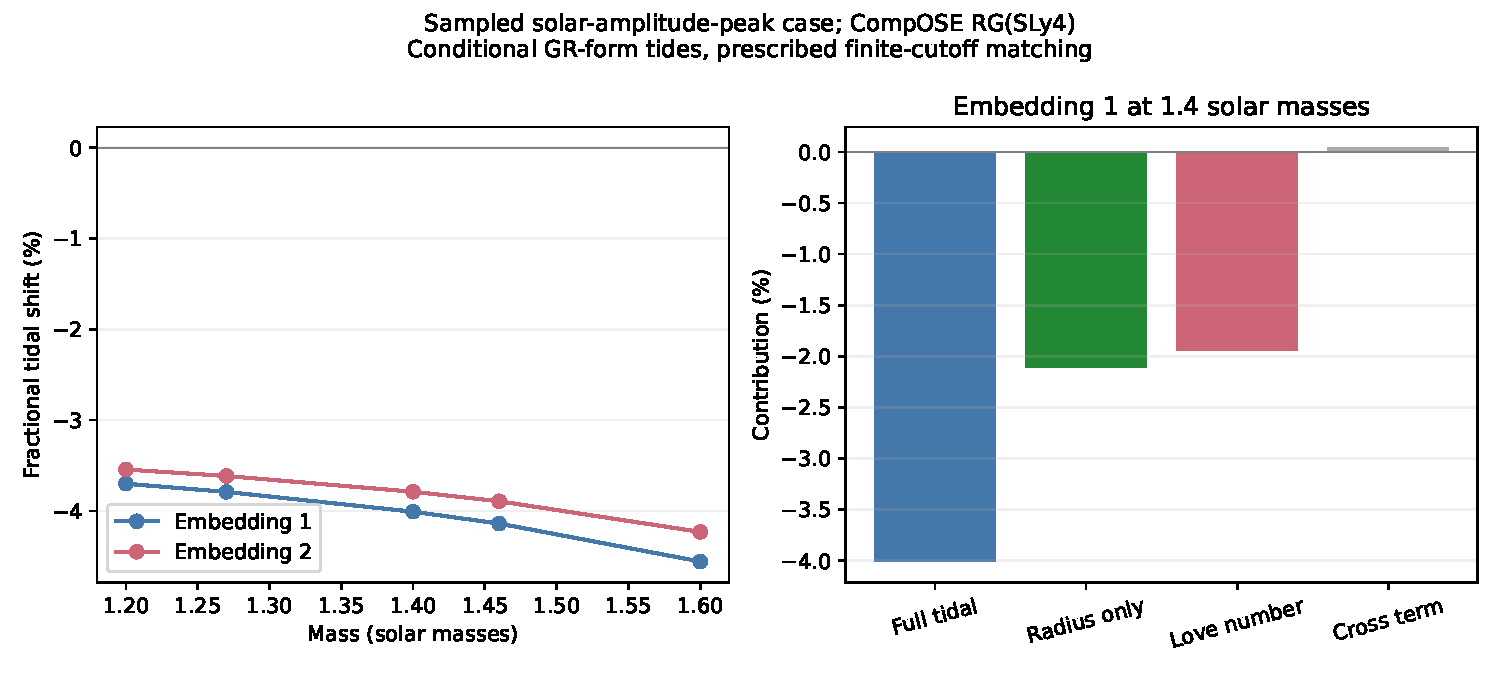
\includegraphics[width=.94\textwidth]{tidal_response.pdf}
\caption{Left: sampled fractional tidal shifts at the common solar point;
lines connect samples rather than define a bound. Right: Embedding~1 at
$1.4M_\odot$, separating the full tidal response, exact radius-only change,
Love-number change and multiplicative cross term. The binary combination is reported separately.}
\label{fig:tides}
\end{figure*}

\section{Numerical verification}
The primary calculation resolves every EOS pressure knot in
$t=\ln(P_c/P)$ and uses the analytic derivative of the selected log-linear
energy interpolant. It does not extrapolate or use a derivative stencil
outside the table. DOP853 settings are rtol $2\times10^{-9}$,
background atol $10^{-17}$, tidal atol $2\times10^{-11}$, maximum step
.08 and central radius 100 cm. Fixed masses are rooted with the checked
background; augmented mass and radius must agree fractionally within
$5\times10^{-7}$, and target masses within $5\times10^{-7}M_\odot$.
Failed integrations and invalid inputs stop admission rather than being
silently skipped.

The Newtonian $n=1$ polytrope, extrapolated from compactness .002, .004
and .008, gives $k_2(0)=.2599086282$ against the analytic .2599088773.
An incompressible extraction check tends to .75. The GR $1.4M_\odot$
result is $R=\GRRadius$ km, $k_2=\GRLove$ and
$\Lambda=\GRLambda$. Both embeddings at $A=0$ and the linear-$H$
form pass the fixed relative $10^{-6}$ tidal gate. Invalid-input and
injected-failure tests also pass.

The retained dataset contains 60 augmented stellar outputs, 21 paired
comparisons and 24 controls, plus background-root evaluations. Three
selected pairs (the solar peak in both embeddings and low alpha in
Embedding~1) each undergo eight controls. Maximum changes in fractional
$\Lambda$ shift are:
\begin{center}
\small\setlength{\tabcolsep}{4pt}
\begin{tabular}{lr}
\hline\hline
Control & Maximum change \\
\hline
Tight integration & $2.314\times10^{-9}$ \\
Linear-$H$, tight integration & $2.314\times10^{-9}$ \\
Start radius 10 / 1,000 cm & $(2.928,3.080)\times10^{-9}$ \\
PCHIP EOS interpolation & $1.616\times10^{-5}$ \\
Surface at $10/100P_{\min}$ & $(1.482,4.092)\times10^{-5}$ \\
Unmodified Einstein $\nu'$ diagnostic & $1.342\times10^{-3}$ \\
\hline\hline
\end{tabular}
\end{center}
Tight settings use rtol $2\times10^{-11}$, background atol $10^{-19}$
and maximum step .03. The first two controls meet the predefined
$10^{-6}$ paired admission threshold. EOS/surface changes are separate
scope sensitivities. The last diagnostic deliberately changes the metric
coefficient in the tidal operator while keeping the background fixed;
it breaks the chosen hydrostatic relation and is not a self-consistent
alternative theory or a theory-error estimate.

\section{Results}
\subsection{Sampled tidal response}
The five main masses at Eq.~(\ref{eq:point}) are shown in
Table~\ref{tab:tides}. Other pairs sample exponents .02, .5 and the
Paper~III NS-extremum slice, reference lengths 5/20 km and the historical
(.0087,.122) point. No tidal-domain extremum or continuous envelope is
certified.




At $1.4M_\odot$, Embedding~1 changes $\Lambda$ by
$\TidalShiftOne\%$. Its radius changes $\RadiusShiftOne\%$ and
its Love number changes $\LoveShiftOne\%$. The exact identity is
\begin{equation}
 \frac{\Lambda_{\rm mod}}{\Lambda_{\rm GR}}=
 \frac{k_{2,\rm mod}}{k_{2,\rm GR}}
 \left(\frac{R_{\rm mod}}{R_{\rm GR}}\right)^5
 \left(\frac{M_{\rm GR}}{M_{\rm mod}}\right)^5.
\end{equation}
The tiny actual mass-root residual is retained. The radius-only tidal
change is $\RadiusOnlyOne\%$, and the radius--Love cross term is
$+\CrossTermOne$ percentage points. Thus $5\Delta R/R+\Delta k_2/k_2$
is only a first-order approximation. Embedding~2 gives
$\Lambda_{1.4}=\LambdaTwo$ and $\TidalShiftTwo\%$; the difference
between embeddings is not an exhaustive uncertainty bound.

\subsection{Shared background and binary example}
Table~\ref{tab:common} repeats the exact common-point record used in
Paper~III. The background domain mass is not a true modified maximum mass:
the sequence reaches the upper EOS edge. Its appearance beside a tidal
value does not remove the exterior assumptions stated above.


For component masses $m_1=1.46M_\odot$ and $m_2=1.27M_\odot$, the usual
mass-weighted combination \cite{Flanagan2008} is
\begin{equation}
 \widetilde\Lambda=\frac{16}{13}
 \frac{(m_1+12m_2)m_1^4\Lambda_1+(m_2+12m_1)m_2^4\Lambda_2}
 {(m_1+m_2)^5}.
\end{equation}
It gives GR $\BinaryGR$, Embedding~1 $\BinaryOne$ and
Embedding~2 $\BinaryTwo$. These replace the rounded 359/345 example.
They are not a new GW170817 likelihood analysis, a detection or a claim
that this model removes EOS/measurement degeneracies. Observational tests
must specify their mass, EOS, waveform and error treatment. The binary
observable is not plotted as though it were a single-star $\Lambda(M)$.

\section{Interpretation and revision history}
The unchanged V6 pipeline at its historical (.0087,.122) point gives a
3.98336\% reduction at $1.4M_\odot$. The checked solver at those same
parameters gives 3.97822\%; the updated solar point gives 4.00852\%.
This separates numerical changes from input changes. V6 used an
uncorrected pressure seed, a finite-difference energy derivative, surface
energy above the cutoff and a zero-pressure jump convention. Its plotting
loop could skip failed stars. Those historical files remain preserved;
they do not supply the current verification evidence.

Earlier force-multiplier enhancements remain results of a different
prescription. The earlier EOS reconstruction error, unsupported APR
predictions and mislabeled Newtonian validation remain withdrawn. Shared
contraction signs are not a criterion for physical validity, and the
current sampled reductions are not universal ceilings.

The calculation now establishes reproducible, numerically controlled
outputs of an explicitly stated conditional tidal prescription. It does
not establish a covariant perturbation sector, a physical surface layer or
smooth matching to the prescribed Schwarzschild exterior. These are
specific unresolved model ingredients, not a requirement for external
endorsement before empirical comparison.

\section*{Code and revision availability}
Producing scripts, inputs, saved results and numerical audit evidence are
publicly available in the \href{https://github.com/chrismerrill1974/solarcore_code/tree/main/reproduction}{shared RDT reproducibility archive}.
The accompanying source package, \nolinkurl{merrill2025_tidal_deformability_code}, includes the
manuscript, dependencies and resource-controlled reproduction commands.
Its \texttt{reproduction/CAPSULE.json} records file hashes;
\texttt{reproduce.py} verifies the package and rebuilds the paper from retained
scientific outputs. Full scientific runs are separate from this saved-result
reproduction. Historical scripts and results remain separately identified.

\section*{Acknowledgments}
Computational collaboration: Astra (Open AI) and Claude (Anthropic).
We thank the developers of NumPy, SciPy and Matplotlib, CompOSE, and the
authors of the EOS tables and tidal-response equations.

\begin{thebibliography}{99}
\bibitem{Hinderer2008}
T.~Hinderer,
``Tidal Love numbers of neutron stars,''
Astrophys. J. \textbf{677}, 1216 (2008);
Erratum: Astrophys. J. \textbf{697}, 964 (2009).

\bibitem{Flanagan2008}
E.~E.~Flanagan and T.~Hinderer,
``Constraining neutron-star tidal Love numbers with gravitational-wave
detectors,''
Phys. Rev. D \textbf{77}, 021502(R) (2008).

\bibitem{PaperI} C.~K.~Merrill, Claude (Anthropic), and Astra (Open AI),
``Radial Dimensionality Theory I: Solar Neutrino and Helioseismic Constraints on Density-Dependent Spatial Dimensionality,''
revised version, November 12, 2026.

\bibitem{WorkingEvidence}
C.~K.~Merrill, Claude (Anthropic), and Astra (Open AI),
RDT working consistency revision: source inputs, numerical audits and
retained scripts, GitHub scientific-input commit \texttt{f4cff7f} (2026),
\href{https://github.com/chrismerrill1974/solarcore_code/tree/main/reproduction}{Shared RDT reproducibility archive}.

\bibitem{PaperIII} C.~K.~Merrill, Claude (Anthropic), and Astra (Open AI),
``Radial Dimensionality Theory III: Neutron Star Structure under Solar-Constrained Density-Dependent Dimensionality,''
revised version, November 12, 2026.

\bibitem{CompOSE}
S.~Typel, M.~Oertel, and T.~Kl\"ahn,
``CompOSE: CompStar online supernova equations of state,''
Phys. Part. Nucl. \textbf{46}, 633 (2015); \url{https://compose.obspm.fr}.

\bibitem{Postnikov2010}
S.~Postnikov, M.~Prakash, and J.~M.~Lattimer,
``Tidal Love numbers of neutron and self-bound quark stars,''
Phys. Rev. D \textbf{82}, 024016 (2010).

\bibitem{Takatsy2020}
J.~Tak\'atsy and P.~Kov\'acs,
``Comment on `Tidal Love numbers of neutron and self-bound quark stars',''
arXiv:2007.01139 (2020), \url{https://arxiv.org/abs/2007.01139}.
\end{thebibliography}
\end{document}
